\documentclass[10pt]{ctexart}
\usepackage{morelull}
\usepackage{enumerate}
\usepackage{bm}
\usepackage{makecell}
\usepackage{xcolor}
\usepackage{graphicx}
\usepackage{subfigure}
\usepackage{framed}%包中有添加文字背景色命令shaded
\colorlet{shadecolor}{MaterialBlue50}
\usepackage{tabularx}
\usepackage{multicol}  
\usepackage{multirow}
\usepackage{indentfirst}
\usepackage{amsmath,amssymb,amsthm,bm,bbding,pifont,dsfont}
\usepackage{mathtools}
\usepackage{tikz}
\newcommand{\abs}[1]{\left| #1 \right|}
\usepackage{caption}
\captionsetup[figure]{labelfont={bf},labelformat={default},labelsep=period,name={图}}
%定义选择题选项
\newcommand{\onech}[4]{
\renewcommand\arraystretch{1.4}
\begin{tabularx}{\linewidth}{XXXX}
\setlength\tabcolsep{0pt}
(A) #1 & (B) #2 & (C) #3 & (D) #4 \\
\end{tabularx}
\unskip \unskip}
\newcommand{\twoch}[4]{
\renewcommand\arraystretch{1.4}
\begin{tabularx}{\linewidth}{XX}
\setlength\tabcolsep{0pt}
(A) #1 & (B) #2 \\
(C) #3 & (D) #4
\end{tabularx}
\unskip \unskip}

%平行四边形
\newcommand*\pxsbx{%
	\mathord{\text{%
			\tikz[baseline]
			\draw (0,.1ex) -- (.8em,.1ex) -- (1em,1.4ex) -- (.2em,1.4ex) -- cycle;}}}

\title{模型研究系列 \quad 蚂蚁行程模型}
\author{一粒沙整理\\安徽省霍邱县龙潭中学}
\date{\today}



\begin{document}
\maketitle
\tableofcontents



\section{立体图形展开的最短路径}
【 {\heiti 模型基础}】

\begin{center}
	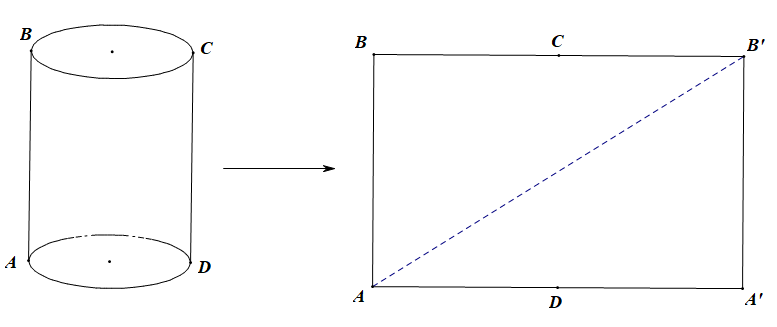
\includegraphics[scale=0.6]{figure/mayixingcheng01}
\end{center}

【 {\heiti 模型分析}】

上图为无底的圆柱体侧面展开图,如图蚂蚁从点$A$沿圆柱表面爬行一周,到点$B$的最短路径就是展开图中$AB'$的长,$AB'=\sqrt{AA'^2+A'B'^2}$。做此类题日的关键就是,正确展开立体图形,利用“两点之间线段最短”或“两边之和大于第三边”准确找出最短路径。

\section{例题学习}

\begin{shaded}
	\begin{example}
	有一圆柱体油罐,已知油罐底面周长是$12m$,高$AB$是$5m$,要从点$A$处开始绕油罐一周建造房子,正好到达$A$点的正上方$B$处,问梯子最短有多长?
	\end{example}
\end{shaded}

\begin{shaded}
	\begin{example}
	如图,一直圆锥的母线长为$QA=8$,底面圆的半径$r=2$, 若一只小蚂蚁从$A$点出发,绕圆锥的侧面爬行一周后又回到$A$点,则蚂蚁爬行的最短路线长是$\underline{\hspace{1.5cm}}$.
	\end{example}
\end{shaded}

\begin{shaded}
	\begin{example}
		已知长方体的长、宽、高分别为$30cm,20cm,10cm$,一只蚂蚁从$A$处出发到$B$处觅食,求它所走的最短路径。(结果保留根号)
	\end{example}
\end{shaded}

\section{模型应用}

\begin{shaded}
1.有一个圆锥体如图,高4cm,底面半径5cm,$A$处有一蚂蚁,若蚂蚁欲沿侧面爬行到$C$处,求蚂蚁爬行的最短距离。
\end{shaded}

\begin{shaded}
2.如图,圆锥体的高为8cm,底面周长为4cm,小蚂蚁在圆柱表面爬行,从$A$点到$B$点,路线如图,则最短路程为$\underline{\hspace{1.5cm}}$.
\end{shaded}

\begin{shaded}
3.桌上有一个圆柱形无盖玻璃杯,高为12厘米,底面周长18厘米,在杯口内壁离杯口距离3厘米的$A$处有一滴蜜糖,一只小虫22 杯子外壁,当它正好在蜜糖相对方向离桌面3厘米的$B$处时,突然发现了蜜糖,问小虫至少爬多少厘米才能到达蜜糖所在的位置。
\end{shaded}

\begin{shaded}
	4.已知$O$为圆锥顶点,$OA,OB$为圆锥的母线,$C$为$OB$的中点,一只小蚂蚁从点$C$开始沿圆锥侧面爬行到点$A$,另一只小蚂蚁也从$C$点出发绕着圆锥侧面爬行到点$B$,它们所爬行的最短路线的痕迹如图所示,若沿$OA$剪开,则得到的圆锥侧面展开图为         (    )
\end{shaded}

\begin{shaded}
	5.如图,一只蚂蚁沿着边长为2的正方体表面从点$A$出发,经过3个面爬行到点$B$,如果它运动的路径是最短的,则最短距离为$\underline{\hspace{1.5cm}}$.
\end{shaded}

\begin{shaded}
6.如图是一个边长为6的正方体木箱,点$Q$在上底面的棱上,$AQ=2$,一只蚂蚁从$P$点出发沿木箱表面爬行到点$Q$,求蚂蚁爬行的最短路线。
\end{shaded}

\begin{shaded}
7.如图,是一个三级台阶,它的每一级的长、宽和高分别等于5cm、3cm和1cm,$A$和$B$是这个台阶的两个相对的端点,$A$点上有一只蚂蚁,想到$B$点去吃可口的食物。请你想一想,这只蚂蚁从$A$点出发,沿着台阶面爬到$B$点的最短路程是多少?
\end{shaded}




\end{document}